\chapter{Introduction}

It is essential that alternatives for electricity production are researched and tested in order to improve efficiencies and reduce the cost of energy. Solar cells are a commonly used form of renewable energy, but are limited by the availability of sunlight. Alternative energy production facilities which use thermal batteries can fill in the power gaps made by other forms which are limited to hour-by-hour availability of resources. This paper explores the relationship between the operating temperature and energy production of a solar thermal Stirling engine and addresses the issues related to the efficiency of such a system.

\section{Stirling Engines}

    Stirling engines are simple heat engines which use the expansion and compression of a gas to create mechanical energy through the irreversible Stirling air cycle \cite{ataer}\cite{chen}. This mechanical energy can then be converted to electrical energy by means of rotational motion and an electric generator. Stirling engines are particularly useful since the energy source is external and can therefore utilize any type of thermal energy.

\section{Solar Thermal Energy}

    Solar thermal electricity generators use solar radiation as the driving heat source for an engine. The process in which these systems typically produce electricity occurs in several steps. A solar concentrator, in most cases a parabolic mirror, focuses sunlight to a pipe in which a liquid salt solution flows \cite{eia:01}. The thermal energy from the light heats the liquid as it flows to a Stirling engine or broiler to produce mechanical power. This mechanical power is then converted to electricity using a generator \cite{ataer}.
    
    \begin{figure}[H]
        \centering
        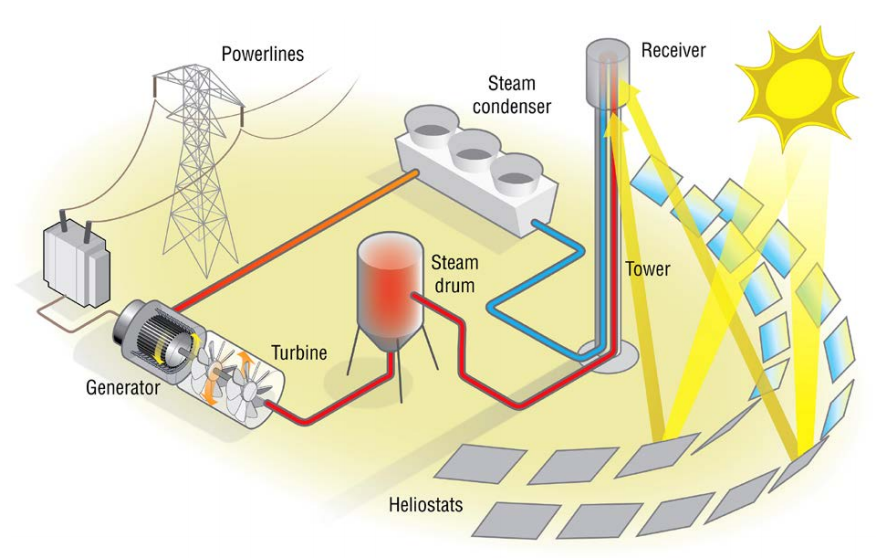
\includegraphics[width=0.75\textwidth]{diagrams/tower}
        \caption[Solar power tower]{Solar power tower diagram. The mirrors focus sunlight to the central tower which houses thermal pipes containing the liquid salt solution. The Ivanpah Solar Power Facility follows this design \cite{tower}.}
        \label{fig:ivanpah}
    \end{figure}
    
    Another system currently in use focuses sunlight with arrays of thousands of mirrors to a single tower which houses the thermal pipes \cite{eia:01}. One such design can be found at the Ivanpah Solar Power Facility near Ivanpah, California\cite{eia:01}, as seen in Figure \ref{fig:ivanpah}. Solar thermal power facilities are also efficient since the energy can be stored in a type of thermal battery which utilizes the heat capacity of the salt solution, reserving the thermal energy to be later converted into mechanical and electrical energy \cite{eia:01}.

\section{Solar Cells}

    Solar thermal engines can be used as an alternative to solar cells for energy production. Solar cells rely on the photovoltaic effect, where a material produces a voltage when exposed to light. However, a large portion of land must be covered with solar cells in order to produce a significant amount of power. This form of alternative energy requires a great deal of maintenance on expensive, inefficient solar cells.
    
    Although sunlight incident to earth includes 77\% of the entire solar spectrum, much less can be converted into usable energy \cite{energyenv}. In practice, around 43\% of the photon energy heats the solar cell \cite{energyenv}. In fact, at 0\degree C, the maximum theoretical efficiency of a solar cell is 24\% \cite{energyenv}. This drops with an increase in operating temperature to just 14\% at 100\degree C \cite{energyenv}. At most times the efficiency hovers between 10-14\% \cite{energyenv}. This is an obvious limitation since solar cells will obviously increase in temperture the longer that they are in operation.
    
    Alternatively, in order to run a large-scale solar thermal electricity generator, there can be one engine and many mirrors to collect the light, such as at Ivanpah. These mirrors are cheaper and require less maintenance than solar cells of equal size and land coverage.